%!TEX root = ../thesis.tex
% ******************************* Thesis Appendix B ****************************
\cleardoublepage
\chapter{Dissimilarity measures between probability distributions}
\label{apx:B}
%*******************************************************************************

Beyond the discrepancy measure to the uniform distribution, this section introduces different dissimilarity measures between probability distributions. 

%============================================================%
%============================================================%
\section*{Csiz\'{a}r $f$-divergences}
%============================================================%
%============================================================%

\elias{General definition}

\elias{Numerous examples depending on the function choosen: see the book culte}

\elias{Link between KL and mutual information}
\elias{Further inputs in the review from Rahman, maybe some in the PhD subject from A.Dutfoy.}
\elias{Problems generated in the estimation}

%============================================================%
%============================================================%
\section*{Integral probability metrics}
%============================================================%
%============================================================%

\elias{general definition}

\elias{Numerous examples see the book culte}

\elias{No closed form expression unlike the $f$-divergence but the use of RKHS goes around this issue.}



%------------------------------------------------------------%
\subsection*{Kernel discrepancy}
%------------------------------------------------------------%
Quasi-Monte Carlo sampling methods widely rely on a uniformity metric, called \textit{discrepancy}. 
This section first presents the link between discrepancy and numerical integration. 
Then it introduces a kernel-based discrepancy, generalizing the concept to non-uniform measures. 
This tool is eventually used to build a sequential quadrature rule by subsampling from a finite dataset.




\paragraph{Reproducing kernel Hilbert space and kernel mean embedding}
%------------------------------------------------------------%
To generalize the Koksma-Hlawka inequality to any probability measure, let us assume that the integrand $g$ lives in a specific function space $\iH(k)$. $\iH(k)$ is a \emph{reproducing kernel Hilbert space} (RKHS), which is an inner product space of functions $g:\iD_{\bX} \rightarrow \R$. 
Considering a symmetric and positive definite function $k: \iD_{\bX} \times \iD_{\bX} \rightarrow \R$, later called a ``reproducing kernel'' or simply a ``kernel'', an RKHS verifies the following axioms: 
\begin{itemize}
    \item The ``feature map'' $\phi : \iD_{\bX} \to \iH(k); \phi(\bx) = k(\cdot, \bx)$ belongs to the RKHS: $k(\cdot, \bx) \in \iH(k), \forall \bx \in \iD_{\bX}$;
    \item The ``reproducing property'': $\langle g, k(\cdot, \bx) \rangle_{\iH(k)} = g(\bx), \quad \forall \bx \in \iD_{\bX}, \forall g \in \iH(k)$.
\end{itemize}
Note that it can be shown that every positive semi-definite kernel defines a unique RKHS (and vice versa) with a feature map $\phi$, such that $k(\bx, \bx') = \langle \phi(\bx), \phi(\bx') \rangle_{\iH(k)}$.
This framework allows us to embed a continuous or discrete probability measure in an RKHS, as illustrated in \fig{fig:kernel_mean_embedding}. 
For any measure $\pi$, let us define its \emph{kernel mean embedding} \citep{sejdinovic_2013}, also called ``potential'' $P_{\pi}(\bx)$ in \cite{pronzato_zhigljavsky_2020}, associated with the kernel $k$ as:

\begin{equation}
   P_{\pi}(\bx) := \int_{\iD_{\bX}} k(\bx, \bx') \dd \pi(\bx').
\end{equation}

Respectively, the potential $P_{\zeta_n}(\bx)$ of a discrete distribution $\zeta_n = \sum_{i=1}^{n} w_i \delta(\bx^{(i)}), w_i \in \R$ associated with the kernel $k$ can be written as:
\begin{equation}\label{eq:potential}
    %P_{\pi}(\bx) := \int_{\iD_{\bX}} k(\bx, \bx') \d \pi(\bx'), \qquad 
    P_{\zeta_n}(\bx) =  \int_{\iD_{\bX}} k(\bx, \bx') \dd \zeta_n(\bx') = \sum_{i=1}^{n} w_i k(\bx, \bx^{(i)}).
\end{equation}
The potential $P_{\pi}(\bx)$ of the targeted measure $\pi$ will be referred to as ``target potential'' and the potential $P_{\zeta_n}(\bx)$ associated with the discrete distribution $\zeta_n$ called ``current potential'' when its support is the current design $\bX_n$. 
When $P_{\zeta_n}(\bx)$ is close to $P_{\pi}(\bx)$, it can be interpreted as $\zeta_n$ being an adequate quantization or representation of $\pi$ (which leads to a good estimation of a quantity such as $I_{\pi}(g)$ from \eq{eq:quadrature_rule}). 
Potentials can be computed in closed forms for specific pairs of distribution and associated kernel. Summary tables of some of these cases are detailed in \cite{briol_phd_2019} (section 3.4), \cite{pronzato_zhigljavsky_2020} (section 4), and extended in \cite{fekhari_iooss_2023}. 
However, in most cases, the target potentials must be estimated on a large and representative sample, typically a large quasi-Monte Carlo sample of $\pi$.

\medskip
\begin{definition}
The \emph{energy} of a measure $\pi$ is defined as the integral of the potential $P_\pi$ against the measure, which leads to the following scalar quantity:
\begin{equation}
    \varepsilon_\pi:= \int_{\iD_{\bX}} P_{\pi}(\bx) \dd \pi(\bx) = \iint_{\iD_{\bX}^2} k(\bx, \bx')\, \dd\pi(\bx) \dd\pi(\bx').
\end{equation}
\label{eq:target_energy}
\end{definition}

\begin{figure}
    \centering
    \begin{tikzpicture}[thick, scale=0.7, every node/.style={transform shape}]
    % Axes
    \def\x{6}\def\y{3.5}
    \draw[-] (-0.5,0) -- (\x+0.5,0) node[right] {};
    \draw[-] (0,-0.5) -- (0,\y+0.5);

    \node (A) at (1.5, 3) {};
    \node (B) at (3.5, 1) {};
    \node (C) at ($(A)!0.5!(B)$) {};
    \draw[{|-|}, very thick] (A) -- (B);

    \fill [red!80] (A) circle (2pt) node[above, black] {$P_{\pi}$};
    \fill [red!80] (B) circle (2pt) node[below, black] {$P_{\zeta}$};
    \node (MMD) at (4.5, 3.5) {$\left\lVert P_{\pi} - P_{\zeta}\right\lVert_{\iH(k)}$};
    \draw[-stealth] (MMD) to [bend left] (C);

    \node [inner sep=0pt] (disc) at (-2,0.9) {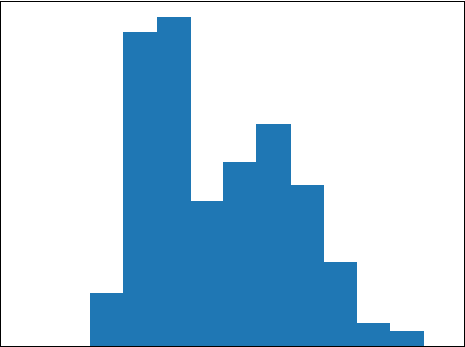
\includegraphics[width=.2\textwidth]{part2/figures/DCE/discrete.pdf}};
    \node [inner sep=0pt] (cont) at (-2,3.1) {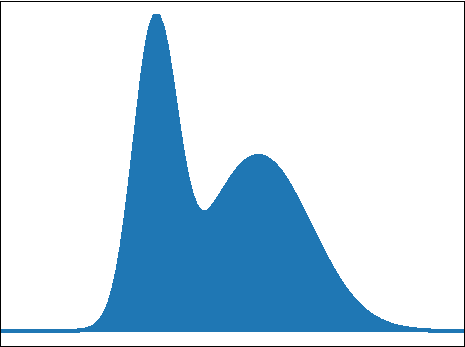
\includegraphics[width=.2\textwidth]{part2/figures/DCE/continuous.pdf}};
    \draw[-stealth] (cont) to [bend left] (A);
    \draw[-stealth] (disc.east) to [bend right] (B);
    % Text
    \node at (5, 0.25) {$\mathcal{H}_k$};
    \node at (-3, 3) {$\pi$};
    \node at (-3, 1) {$\zeta$};
\end{tikzpicture}
    \caption{Kernel mean embedding of a continuous and discrete probability distribution}
    \label{fig:kernel_mean_embedding}
\end{figure}
Finally, using the reproducing property and writing the Cauchy-Schwarz inequality on the absolute quadrature error leads to the following inequality, similar to the Koksma-Hlawka inequality \eq{eq:KH_inequality} (see \cite{briol_oates_2019}): 

\begin{subequations}
\begin{align}
    \left| \sum_{i=1}^{n} w_i g(\bx^{(i)}) - \int_{\iD_{\bX}} g(\bx) \dd \pi(\bx) \right| &= \left| \left\langle g, P_{\zeta_n}(\bx) \right\rangle_{\iH(k)} - \left\langle g, P_{\pi}(\bx) \right\rangle_{\iH(k)} \right| \\
    &= \left| \left\langle g, \left(P_{\zeta_n}(\bx) - P_{\pi}(\bx)\right) \right\rangle_{\iH(k)} \right|\\
    &\leq \lVert g \lVert_{\iH(k)}  \left\lVert P_{\pi}(\bx) - P_{\zeta_n}(\bx) \right\lVert_{\iH(k)}.
    \label{eq:quad_error}
\end{align}
\end{subequations}

\paragraph{Maximum mean discrepancy}
%------------------------------------------------------------%
A metric of discrepancy and quadrature error is offered by the \emph{maximum mean discrepancy} (MMD). 
This distance between two probability distributions $\pi$ and $\zeta$ is given by the worst-case error for any function within a unit ball of the Hilbert space $\iH(k)$, associated with the kernel $k$:
\begin{equation}
    \MMD(\pi, \zeta) := %\\ 
    \sup_{\lVert g \lVert_{\iH(k)} \leq 1}
            \left | \int_{\iD_{\bX}} g(\bx) \dd \pi(\bx) - \int_{\iD_{\bX}} g(\bx) \dd \zeta(\bx) \right| %= \left\lVert P_{\pi}(\bx) - P_{\zeta}(\bx) \right\lVert_{\iH(k)}.
    \label{eq:mmd_c4}  
\end{equation}

According to the inequality in \eq{eq:quad_error}, $\MMD(\pi, \zeta) = \left\lVert P_{\pi} - P_{\zeta} \right\lVert_{\iH(k)}$, meaning that the MMD fully relies on the difference of potentials. 
Moreover, \cite{sriperumbudur_2010} defines a kernel as ``characteristic kernel'' when the following equivalence is true: $\MMD(\pi, \zeta) = 0 \Leftrightarrow \pi = \zeta$. 
This property makes the MMD a metric on $\iD_{\bX}$. 
The squared MMD has been used for other purposes than numerical integration: e.g., statistical testing \citep{gretton_2006}, and global sensitivity analysis \citep{daveiga_2015}. 
It can be written as follows:

\begin{subequations}
\begin{align}
    \MMD(\pi, \zeta)^2 &= \left\lVert P_{\pi}(\bx) - P_{\zeta}(\bx) \right\lVert^2_{\iH(k)}\\
        &= \left\langle \left(P_{\pi}(\bx) - P_{\zeta}(\bx) \right), \left(P_{\pi}(\bx) - P_{\zeta}(\bx) \right) \right\rangle_{\iH(k)}\\
        &= \left\langle P_{\pi}(\bx), P_{\pi}(\bx) \right\rangle_{\iH(k)} - 2 \left\langle P_{\pi}(\bx), P_{\zeta}(\bx) \right\rangle_{\iH(k)} + \left\langle P_{\zeta}(\bx), P_{\zeta}(\bx) \right\rangle_{\iH(k)}\\
        &= \iint_{\iD_{\bX}^2} k(\bx, \bx')\, \dd\pi(\bx) \dd\pi(\bx') - 2 \iint_{\iD_{\bX}^2} k(\bx, \bx')\, \dd\pi(\bx) \dd\zeta(\bx') + \iint_{\iD_{\bX}^2} k(\bx, \bx')\, \dd\zeta(\bx) \dd\zeta(\bx').
\end{align}
\end{subequations}
Taking a discrete distribution with uniform weights $\zeta_n= \frac{1}{n} \sum_{i=1}^{n} \delta(\bx^{(i)})$, the squared MMD reduces to: 
\begin{equation}\label{eq:mmd_design}
    \MMD(\pi, \zeta_n)^2 = \varepsilon_\pi - \frac{2}{n} \sum_{i=1}^n P_{\pi}\left(\bx^{(i)}\right) + \frac{1}{n^2} \sum_{i, j=1}^n k\left(\bx^{(i)}, \bx^{(j)}\right).
\end{equation}
%\begin{remark}
% Should we compare MMD to other divergences (see Sriperumbudur 2010)?
%A strong link exists between numerical integration and space-filling design of experiments. The MMD yields an upper bound over a geometric space-filling metric called the ``covering radius'' (see section 4.1.2 in \cite{pronzato_zhigljavsky_2020}). 
%\end{remark}





%============================================================%
\subsection*{Maximum discrepancy measure}
%============================================================%

A metric of discrepancy between distributions is introduced as the \emph{maximum mean discrepancy} (MMD). 
This distance between two probability distributions $\mu$ and $\zeta$ is defined as the worst-case error for any function within a unit ball of a function space $\iH$:
\begin{equation}
    \MMD(\mu, \zeta) := %\\ 
    \sup_{\lVert g \lVert_{\iH} \leq 1}
            \left | \int_{\iD_{\bX}} g(\bx) \dd \mu(\bx) - \int_{\iD_{\bX}} g(\bx) \dd \zeta(\bx) \right| = \left\lVert P_{\mu}(\bx) - P_{\zeta}(\bx) \right\lVert_{\iH}.
    \label{eq:mmd}  
\end{equation}

To ease the calculation of the quantity, this metric was studied for a particular function space, offering specific properties.
A \emph{reproducing kernel Hilbert space} (RKHS), denoted $\iH(k)$, is an inner product space $\iH(k)$ of functions $g:\iD_{\bX} \rightarrow \R$.
It verifies the following axioms, considering a symmetric and positive definite function $k: \iD_{\bX} \times \iD_{\bX} \rightarrow \R$, later called a ``reproducing kernel'' or simply a ``kernel'': 
\begin{itemize}
    \item The ``feature map'' $\phi : \iD_{\bX} \to \iH(k); \phi(\bx) = k(\cdot, \bx) \in \iH(k), \forall \bx \in \iD_{\bX}$.
    \item The ``reproducing property'': $\langle g, k(\cdot, \bx) \rangle_{\iH(k)} = g(\bx), \quad \forall \bx \in \iD_{\bX}, \forall g \in \iH(k)$.
\end{itemize}
Every positive semi-definite kernel defines a unique RKHS (and vice versa) with a feature map $\phi$, such that $k(\bx, \bx') = \langle \phi(\bx), \phi(\bx') \rangle_{\iH(k)}$.
Moreover, \cite{sriperumbudur_2010} defines a kernel as ``characteristic kernel'' when the following equivalence is true: $\MMD_k(\mu, \zeta) = 0 \Leftrightarrow \mu = \zeta$. 
This property makes the MMD a metric on $\iD_{\bX}$.

Then, a probability measure has a representation in the RKHS through its \emph{kernel mean embedding} \citep{sejdinovic_2013}, also called ``potential'' $P_{\mu}(\bx)$ in \cite{pronzato_zhigljavsky_2020}, defined as:
\begin{equation}
   P_{\mu}(\bx) := \int_{\iD_{\bX}} k(\bx, \bx') \dd \mu(\bx').
\end{equation}
The reproducing property from the RKHS allows to express the squared MMD as expectations of kernels:
\begin{equation}\label{eq:mmd2}
    \MMD_k(\mu, \zeta)^2 = \int_{\iD_{\bX}} P_{\mu}(\bx)\, \dd\mu(\bx) - 2 \int_{\iD_{\bX}} P_{\mu}(\bx) \, \dd\zeta(\bx) + \int_{\iD_{\bX}} P_{\zeta}(\bx)\, \dd\zeta(\bx).
\end{equation}

\elias{Add a sentence on estimation}


%%%%%%%%%%%%%%%%%%%%%%%%%%%%%%%%%%%%%%%%%%%%%%%
\subsection*{Analytical computation of potentials for Mat\'ern kernels}

As for tensor-product kernels, the potential is the product of the one-dimensional potentials, we only consider one-dimensional input spaces.

For $\mu$ the uniform distribution on $[0,1]$ and $K$ the Matérn kernel $K_{5/2,\theta}$ with smoothness $\nu=5/2$ and correlation length $\theta$, see \eqref{eq:Matern5/2}, we get
\bea
    P_{K_{5/2,\theta},\mu}(x) = \frac{16 \theta}{3 \sqrt{5}} - \frac{1}{15 \theta} (S_\theta(x) + S_\theta(1-x)),
\eea
where
% \begin{equation}
% \nonumber
%     S_\theta(x) = \frac{1}{15} \left[ \exp\left(- \frac{\sqrt{5}}{\theta} x \right) 
%     \left( - \frac{5}{\theta} x \left( \frac{\sqrt{5}}{\theta} x + 5 \right) - 8 \sqrt{5} \right)
%     + 8 \sqrt{5} \right].
% \end{equation}
\bea
\nonumber
    S_\theta(x) = 
    \exp\left(- \frac{\sqrt{5}}{\theta} x \right) 
    \left( 5 \sqrt{5} x^2 + 25 \theta x + 8 \sqrt{5} \theta^2 \right).
\eea
The expressions $P_{K_{\nu,\theta},\mu}(x)$ for $\nu=1/2$ and $\nu=3/2$ can be found in \cite{prozhi20}. 

When $\mu$ is the standard normal distribution $\mathcal{N}(0,1)$, the potential $P_{K_{5/2,\theta},\mathcal{N}(0,1)}$ is 
%\bea
$    P_{K_{5/2,\theta},\mathcal{N}(0,1)}(x) = T_\theta(x) + T_\theta(-x),
$
%\eea
where
\bea
T_\theta(x) &=&
    \frac{1}{6} 
    \left( 
        \frac{5}{\theta^2} x^2 + 
        \left( 3 - \frac{10}{\theta^2} \right) \frac{\sqrt{5}}{\theta} x + \frac{5}{\theta^2} \left( \frac{5}{\theta^2} -2 \right) + 3
    \right) \\
    && \times\, \mathrm{erfc} \left( \frac{\frac{\sqrt{5}}{\theta} - x}{\sqrt{2}} \right)
    \exp\left(\frac{5}{2 \theta^2} - \frac{\sqrt{5}}{\theta}x\right) + \frac{1}{3 \sqrt{2 \pi}} \frac{\sqrt{5}}{\theta} 
    \left( 3 - \frac{5}{\theta^2} \right) \exp\left(-\frac{x^2}{2}\right). 
\eea
